\documentclass[letterpaper, 10pt, conference]{ieeeconf}
\IEEEoverridecommandlockouts
\overrideIEEEmargins

\usepackage{amsmath,amssymb}
\usepackage{graphicx}
\usepackage{booktabs}
\usepackage{xurl}
\usepackage[hidelinks]{hyperref}
\usepackage{tikz}
\usetikzlibrary{arrows.meta}

\hyphenpenalty=10000
\exhyphenpenalty=10000
\emergencystretch=2em
\raggedbottom

\newcommand{\code}[1]{\texttt{#1}}
\newcommand{\p}{\mathbf{p}}
\newcommand{\q}{\mathbf{q}}
\newcommand{\tb}{\mathbf{t}}
\newcommand{\x}{\mathbf{x}}
\newcommand{\step}[1]{\par\noindent\textit{Step #1.}\ }

\begin{document}

\title{ECE 276A Project 2: LiDAR-Based SLAM}

\author{\authorblockN{Aditya Wirayutha Kaya Simto}
\authorblockA{Department of Computer Science and Systems Engineering \\ Kobe University}}

\maketitle
\thispagestyle{empty}
\pagestyle{empty}

%======================================================================
\section{Introduction}

Indoors there is no GPS, and odometry drifts: on dataset 20 it ends 2.77\,m
from the start after a 95.9\,m drive. SLAM (Simultaneous Localization and
Mapping) estimates the path and the map together, so that seeing the same
wall twice corrects the path.

The system has four stages for a differential-drive robot with encoders, an
IMU, a 2-D LiDAR and a Kinect~\cite{atanasov} (Fig.~\ref{fig:pipeline}):
(1)~encoder and IMU odometry, (2)~ICP scan matching, (3)~pose graph
optimization with loop closures in GTSAM~\cite{gtsam}, and (4)~occupancy grid
and floor texture mapping with the optimized poses. The final path ends
0.12\,m (dataset 20) and 0.22\,m (dataset 21) from the start, compared to 2.7
to 3.3\,m for odometry or ICP alone.

%======================================================================
\section{Problem Formulation}

\emph{Pose.} $\x=(x,y,\theta)$ with $\theta\in[-\pi,\pi)$, and matrix form
\begin{equation}
T(\x)=\begin{bmatrix}R(\theta) & \tb\\ \mathbf{0}^\top & 1\end{bmatrix}
=\begin{bmatrix}\cos\theta & -\sin\theta & x\\ \sin\theta & \cos\theta & y\\ 0&0&1\end{bmatrix},
\end{equation}
which maps a body point to the world: $\p_W=R\p_B+\tb$. The pose of $j$
relative to $i$ is $T_i^{-1}T_j$. For scan $k$, $T_k=T(\x_k)$ has rotation
$R_k=R(\theta_k)$ and translation $\tb_k$. The unknowns are the path
$\{\x_0,\dots,\x_K\}$ (one pose per LiDAR scan), the occupancy map $m$ and
the floor color map $c$.

\emph{Motion model.} With speed $v_t$, yaw rate $\omega_t$, time step $\tau_t$:
\begin{equation}
\theta_{t+1}=\theta_t+\omega_t\tau_t,\quad
\begin{bmatrix}x_{t+1}\\y_{t+1}\end{bmatrix}=\begin{bmatrix}x_t\\y_t\end{bmatrix}+v_t\tau_t\begin{bmatrix}\cos\theta_{t+1}\\\sin\theta_{t+1}\end{bmatrix}.
\label{eq:motion}
\end{equation}

\emph{Registration.} For point sets $\{\p_k\}$, $\{\q_k\}$ with known pairs,
\begin{equation}
\begin{gathered}
(R^*,\tb^*)=\arg\min_{R,\,\tb}\ \sum_{k=1}^{N} \lVert \q_k-(R\p_k+\tb)\rVert^2\\
\text{subject to}\quad R^\top R=I,\ \det R=1.
\end{gathered}
\label{eq:registration}
\end{equation}
ICP solves the same problem when the pairs are unknown.

\emph{Pose graph.} Each edge $(i,j)\in\mathcal{E}$ carries a measured
relative pose $\mathbf{u}_{ij}=(\mathbf{u}^{xy}_{ij},u^{\theta}_{ij})$ (pose
$j$ seen from pose $i$, from ICP) with covariance $\Sigma_{ij}$ and
information matrix $\Omega_{ij}=\Sigma_{ij}^{-1}$. Composing pose $i$ with the
measurement predicts pose $j$:
\begin{equation}
f(\x_i,\mathbf{u}_{ij})=\begin{bmatrix}\tb_i+R(\theta_i)\,\mathbf{u}^{xy}_{ij}\\ \theta_i+u^{\theta}_{ij}\end{bmatrix},\qquad
\mathbf{e}_{ij}=\x_j-f(\x_i,\mathbf{u}_{ij}),
\label{eq:residual}
\end{equation}
with the angle entry of $\mathbf{e}_{ij}$ wrapped to $[-\pi,\pi)$. The
estimate minimizes
\begin{equation}
\x^*=\arg\min_{\x}\ \mathcal{J}(\x),\qquad
\mathcal{J}(\x)=\tfrac12\sum_{(i,j)\in\mathcal{E}}\mathbf{e}_{ij}^\top\Omega_{ij}\,\mathbf{e}_{ij}.
\label{eq:posegraph}
\end{equation}
GTSAM's \code{Pose2} factor writes the same error rotated into the frame of
the prediction, which leaves $\mathcal{J}$ unchanged because
$\sigma_x=\sigma_y$ for every edge.

\emph{Occupancy grid.} Each cell $m_i$ holds the log-odds
$\lambda_i=\log\frac{p(m_i=1\mid z_{1:t})}{p(m_i=0\mid z_{1:t})}$, with
$\lambda_i=0$ meaning unknown (50\,\%).

%======================================================================
\section{Technical Approach}

Table~\ref{tab:functions} gives the input and output of each function in the
code.

\begin{table*}[t]
\caption{Functions in \code{main.py} and \code{icp.py}. $N$ = number of points, $K$ = number of LiDAR scans (4962 for dataset 20).}
\label{tab:functions}
\centering
\small
\begin{tabular}{@{}lp{0.23\textwidth}p{0.40\textwidth}@{}}
\toprule
Function & Input & Returns \\
\midrule
\code{odometry(d)} & sensor data & (4956, 3) array of $(x,y,\theta)$, one per encoder reading \\
\code{lidar\_points(d, k)} & scan number $k$ & (N, 2) points of scan $k$ in the body frame (meters) \\
\code{kabsch(P, Q)} & two (N, d) arrays, row $k$ paired with row $k$ & \code{R, t, rmsd}: best rotation, translation, fit error \\
\code{icp(source, target, T\_initial)} & two clouds, no pairs, a starting guess & \code{T, error}: $(d{+}1)\times(d{+}1)$ transform source$\to$target, mean pair distance \\
\code{scan\_matching(d, odom)} & data, odometry poses & (K, 3) poses, one per LiDAR scan \\
\code{match\_scans(d, poses\_T, i, j, \dots)} & two scan numbers & \code{T\_relative, inlier\_ratio}: pose of $j$ relative to $i$, share of points within 10\,cm \\
\code{pose\_graph(d, icp\_poses)} & data, (K, 3) ICP poses & (K, 3) optimized poses \\
\code{occupancy\_map(d, poses)} & data, (K, 3) poses & \code{map\_info, grid, snapshots}: 1600$\times$1600 log-odds grid + 4 copies over time \\
\code{camera\_to\_body()} & none & $3\times3$ rotation, Kinect frame $\to$ body frame \\
\code{texture\_map(d, dataset, poses)} & data, poses & \code{map\_info, texture, snapshots}: 1600$\times$1600$\times$3 color image + 4 copies \\
\bottomrule
\end{tabular}
\end{table*}

\begin{figure}[t]
\centering
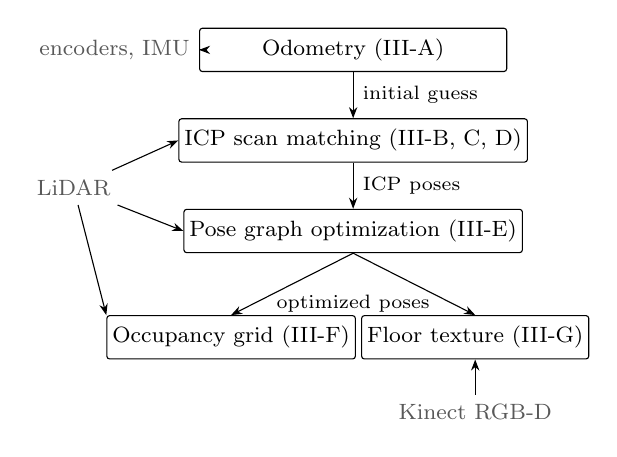
\begin{tikzpicture}[font=\footnotesize, >={Stealth[length=4pt]},
  stage/.style={draw, rounded corners=1pt, minimum height=0.55cm, align=center, inner sep=2pt},
  sensor/.style={text=black!65, align=center}]
\node[stage, minimum width=3.9cm] (odo) at (4.4,0) {Odometry (III-A)};
\node[stage, minimum width=3.9cm] (sm) at (4.4,-1.15) {ICP scan matching (III-B, C, D)};
\node[stage, minimum width=3.9cm] (pg) at (4.4,-2.3) {Pose graph optimization (III-E)};
\node[stage, minimum width=2.6cm] (occ) at (2.85,-3.65) {Occupancy grid (III-F)};
\node[stage, minimum width=2.6cm] (tex) at (5.95,-3.65) {Floor texture (III-G)};
\node[sensor, anchor=east] (enc) at (2.45,0) {encoders, IMU};
\node[sensor] (lid) at (0.85,-1.75) {LiDAR};
\node[sensor] (kin) at (5.95,-4.6) {Kinect RGB-D};
\draw[->] (enc) -- (odo);
\draw[->] (odo) -- node[right, font=\scriptsize] {initial guess} (sm);
\draw[->] (sm) -- node[right, font=\scriptsize] {ICP poses} (pg);
\draw[->] (pg.south) -- (occ.north);
\node[font=\scriptsize] at (4.4,-3.22) {optimized poses};
\draw[->] (pg.south) -- (tex.north);
\draw[->] (lid) -- (sm.west);
\draw[->] (lid) -- (pg.west);
\draw[->] (lid) -- (occ.north west);
\draw[->] (kin) -- (tex);
\end{tikzpicture}
\caption{Pipeline. Labels give the subsections of Section~III.}
\label{fig:pipeline}
\end{figure}

%----------------------------------------------------------------------
\subsection{Odometry}

\step{1} Distance per tick, wheel diameter $D=0.254$\,m, 360 ticks per turn:
$s=\pi D/360\approx0.0022$\,m.

\step{2} Side travel from the counts $FR,FL,RR,RL$ since the last reading:
\begin{equation}
d_R=\tfrac{FR+RR}{2}\,s,\qquad d_L=\tfrac{FL+RL}{2}\,s.
\end{equation}

\step{3} The center of a differential-drive robot moves by the average of
the two sides, so with $\tau$ the encoder time step,
\begin{equation}
l=\tfrac{d_R+d_L}{2},\qquad v=\tfrac{l}{\tau}.
\end{equation}

\step{4} Yaw rate: the wheels give $\omega=(d_R-d_L)/(b\,\tau)$ with track
width $b$, but wheels slip in turns, so $\omega$ is taken from the IMU
$z$-axis gyro at the nearest IMU time stamp.

\step{5} Integrate with the Euler step~\eqref{eq:motion}, assuming $v$ and
$\omega$ constant over each $\tau$.

%----------------------------------------------------------------------
\subsection{Kabsch algorithm (known pairs)}

\step{1} Objective~\eqref{eq:registration}:
$E(R,\tb)=\sum_k\lVert\q_k-R\p_k-\tb\rVert^2$.

\step{2} Optimal translation. Setting the gradient to zero,
\begin{equation}
\frac{\partial E}{\partial\tb}=-2\sum_k(\q_k-R\p_k-\tb)=0
\;\Rightarrow\;
\tb^*=\bar{\q}-R\bar{\p},
\end{equation}
with centroids $\bar{\p}=\frac1N\sum_k\p_k$, $\bar{\q}=\frac1N\sum_k\q_k$.
This is why centroids are used: the best translation always moves the
source centroid onto the target centroid, so after centering both sets the
translation drops out and the rotation can be solved alone.

\step{3} Centered points $\p'_k=\p_k-\bar{\p}$, $\q'_k=\q_k-\bar{\q}$.
Substituting $\tb^*$ and expanding, with $\lVert R\p'_k\rVert=\lVert\p'_k\rVert$:
\begin{equation}
E(R)=\sum_k\big(\lVert\q'_k\rVert^2+\lVert\p'_k\rVert^2\big)-2\sum_k\q'^\top_kR\,\p'_k .
\end{equation}
The first sum does not depend on $R$, so minimizing $E$ means maximizing the
last sum.

\step{4} Trace form. Since $\q'^\top R\p'=\operatorname{tr}(R\,\p'\q'^\top)$,
\begin{equation}
\begin{aligned}
\textstyle\sum_k\q'^\top_kR\,\p'_k&=\operatorname{tr}(RH),\\
H&=\textstyle\sum_k\p'_k\q'^\top_k=P'^\top Q'\in\mathbb{R}^{d\times d}.
\end{aligned}
\end{equation}

\step{5} SVD. Every real matrix factors as
\begin{equation}
\begin{gathered}
H=U\Sigma V^\top,\quad U^\top U=V^\top V=I,\\
\Sigma=\operatorname{diag}(\sigma_1\ge\dots\ge\sigma_d\ge0),
\end{gathered}
\end{equation}
i.e.\ a rotation (or reflection), a scaling along the axes, and another
rotation. $\sigma_i$ are the singular values.

\step{6} Bound. By the cyclic property of the trace,
\begin{equation}
\begin{aligned}
\operatorname{tr}(RH)&=\operatorname{tr}(RU\Sigma V^\top)=\operatorname{tr}(\Sigma\,V^\top RU)\\
&=\textstyle\sum_i\sigma_iM_{ii},\qquad M=V^\top RU.
\end{aligned}
\end{equation}
$M$ is orthogonal, so $|M_{ii}|\le1$ and $\operatorname{tr}(RH)\le\sum_i\sigma_i$.
Equality holds for $M=I$, so $R^*=VU^\top$.

\step{7} Reflection fix. If $\det(VU^\top)=-1$, $VU^\top$ is a mirror, not a
rotation. The best proper rotation flips the axis with the smallest
$\sigma_d$:
\begin{equation}
R^*=V\operatorname{diag}\!\big(1,\dots,1,\det(VU^\top)\big)U^\top,
\end{equation}
which the code does by negating the last row of $V^\top$. A self-test
rotates a random cloud by $40^\circ$ and recovers $R$ and $\tb$ exactly.

%----------------------------------------------------------------------
\subsection{ICP (unknown pairs)}

\step{1} Start from $T^0$ and build a KD-tree on the target once.

\step{2} Transform: $\tilde\p_k=R^n\p_k+\tb^n$.

\step{3} Correspondence (nearest neighbor):
\begin{equation*}
j(k)=\arg\min_j\lVert\q_j-\tilde\p_k\rVert .
\end{equation*}

\step{4} Outlier rejection:
\begin{equation*}
\mathcal{I}=\{k:\lVert\q_{j(k)}-\tilde\p_k\rVert<d_{\max}\}.
\end{equation*}

\step{5} Update with Kabsch on the kept pairs:
\begin{equation*}
(R^{n+1},\tb^{n+1})=\text{Kabsch}\big(\{\p_k,\q_{j(k)}\}_{k\in\mathcal{I}}\big).
\end{equation*}

\step{6} Error and stopping rule:
\begin{equation*}
\begin{gathered}
e^n=\frac{1}{|\mathcal{I}|}\sum_{k\in\mathcal{I}}\lVert\q_{j(k)}-\tilde\p_k\rVert,\\
\text{stop if }|e^{n-1}-e^n|<10^{-6}\ \text{or}\ n=50.
\end{gathered}
\end{equation*}

\emph{Convergence.} With $E(T,j)$ the error for transform $T$ and pairing $j$,
\begin{equation}
E(T^n,j^n)\ \ge\ E(T^n,j^{n+1})\ \ge\ E(T^{n+1},j^{n+1}),
\end{equation}
because step 3 picks the closest pairs for the current $T$ and step 5 picks
the best $T$ for those pairs. A non-increasing sequence bounded below by 0
converges, so ICP stops, but only at the nearest local minimum. A far-off
$T^0$ gives wrong pairs from the first iteration, so a good initial guess is
required. (With $d_{\max}$ the kept set changes, so the decrease is nearly,
not strictly, monotone.)

\emph{Warm-up.} The partial view is registered onto the full model and the
result inverted: every view point has a partner on the model, but the
hidden back of the model has none in the view. ICP is started from 12 yaws
($0^\circ,30^\circ,\dots,330^\circ$), each with the centroids aligned, using
every 10th view point; the start with the lowest error is refined with all
view points.

%----------------------------------------------------------------------
\subsection{LiDAR scan matching}

\step{1} Ranges to body points: for beam $n$ with range $r_n$,
$\alpha_n=\alpha_{\min}+n\Delta\alpha$ and
\begin{equation}
\p_n=\big(r_n\cos\alpha_n+0.133,\ r_n\sin\alpha_n\big),\quad r_{\min}<r_n<r_{\max},
\end{equation}
where $0.133$\,m (0.13323 in the code) is the LiDAR offset from the robot
center~\cite{config}. $S_k=\{\p_n\}$ is the point set of scan $k$.

\step{2} Relative pose. A wall point has one world position:
$T_i\p^{(i)}=T_j\p^{(j)}\Rightarrow\p^{(i)}=(T_i^{-1}T_j)\,\p^{(j)}$. So ICP of
scan $j$ onto scan $i$ estimates $T_i^{-1}T_j$.

\step{3} Initial guess from odometry poses $O$, relative to keyframe $\text{kf}$:
\begin{equation}
T^0=T_{\text{kf}}^{-1}\,T_{k-1}\,(O_{k-1}^{-1}O_k).
\end{equation}
$O_{k-1}^{-1}O_k$ is the odometry step in the robot frame, so it can be
stacked on the ICP pose $T_{k-1}$ even after the two paths drift apart.

\step{4} Match and compose:
$T_{\text{rel}}=\text{ICP}(S_k,S_{\text{kf}},T^0)$, $T_k=T_{\text{kf}}T_{\text{rel}}$.

\step{5} Scan $k$ becomes the keyframe when $\lVert\tb_{\text{rel}}\rVert>0.5$\,m
or $|\theta_{\text{rel}}|>0.2$\,rad. Consecutive scans are only 2\,cm apart;
ICP under-reports such a small motion in a hallway, and chaining 4962 such
steps made the hallways too short.

%----------------------------------------------------------------------
\subsection{Pose graph optimization}

\step{1} Variables: $\x=(\x_0,\dots,\x_K)$, initialized with the ICP poses.

\step{2} Edges $\mathcal{E}$, each with $\mathbf{e}_{ij}$ from \eqref{eq:residual}:
\begin{itemize}
\item prior on $\x_0$: $\mathbf{e}_0=\x_0-\bar{\x}_0$ ($\bar{\x}_0$ the first ICP pose), $\sigma=10^{-3}$;
\item odometry $(k-1,k)$: $\mathbf{u}$ = ICP step $T_{k-1}^{-1}T_k$,
      $\sigma=(0.01,0.01,0.005)$;
\item fixed-interval loops $(i,i+10)$, ICP with $d_{\max}=0.5$\,m;
\item proximity loops $(i,j)$, every 20th scan, $\lVert\tb_i-\tb_j\rVert<2$\,m
      and $j-i\ge500$, ICP with $d_{\max}=1.0$\,m.
\end{itemize}
A loop edge $\mathbf{u}_{ij}=\text{ICP}(S_j,S_i,T_i^{-1}T_j)$ is kept only if
its inlier ratio
\begin{equation}
\rho_{ij}=\frac1N\sum_k\mathbf{1}\Big[\min_{\q\in S_i}\lVert U_{ij}\p_k-\q\rVert<0.1\Big]\ge0.6,
\end{equation}
with $U_{ij}$ the matrix form of $\mathbf{u}_{ij}$. Loop edges use
$\sigma=(0.1,0.1,0.05)$.

\step{3} Robust cost. With the whitened error
$\varepsilon_{ij}=\sqrt{\mathbf{e}_{ij}^\top\Omega_{ij}\mathbf{e}_{ij}}$,
\begin{equation}
\begin{gathered}
\mathcal{J}(\x)=\sum_{\text{prior, odo}}\tfrac12\varepsilon_{ij}^2+\sum_{\text{loop}}\rho_H(\varepsilon_{ij}),\\
\rho_H(\varepsilon)=\begin{cases}\tfrac12\varepsilon^2,&\varepsilon\le1\\ \varepsilon-\tfrac12,&\varepsilon>1\end{cases}
\end{gathered}
\end{equation}
$\rho_H$ grows linearly for large $\varepsilon$, so a wrong loop pulls with
bounded force.

\step{4} Linearize around the current estimate $\x^{(n)}$:
$\mathbf{e}_{ij}(\x^{(n)}+\delta\x)\approx\mathbf{e}_{ij}+J_i\,\delta\x_i+J_j\,\delta\x_j$.
Differentiating \eqref{eq:residual}, with
$\frac{d}{d\theta}R(\theta)=R(\theta)S$ and $S=\left[\begin{smallmatrix}0&-1\\1&0\end{smallmatrix}\right]$,
\begin{equation}
J_i=\frac{\partial\mathbf{e}_{ij}}{\partial\x_i}=
\begin{bmatrix}-I_2 & -R(\theta_i)S\,\mathbf{u}^{xy}_{ij}\\ \mathbf{0}^\top & -1\end{bmatrix},\qquad
J_j=\frac{\partial\mathbf{e}_{ij}}{\partial\x_j}=I_3 .
\end{equation}

\step{5} Quadratic model and its minimum. Substituting into
\eqref{eq:posegraph} and setting the gradient with respect to $\delta\x$
to zero gives the normal equations $H\,\delta\x=-\mathbf{b}$, assembled edge by
edge:
\begin{equation}
\begin{aligned}
H_{ii}&\mathrel{+}=J_i^\top\Omega_{ij}J_i, & H_{ij}&\mathrel{+}=J_i^\top\Omega_{ij}J_j,\\
H_{ji}&\mathrel{+}=J_j^\top\Omega_{ij}J_i, & H_{jj}&\mathrel{+}=J_j^\top\Omega_{ij}J_j,\\
\mathbf{b}_i&\mathrel{+}=J_i^\top\Omega_{ij}\mathbf{e}_{ij}, & \mathbf{b}_j&\mathrel{+}=J_j^\top\Omega_{ij}\mathbf{e}_{ij}.
\end{aligned}
\end{equation}
The prior adds $\Omega_0$ to $H_{00}$ and $\Omega_0\mathbf{e}_0$ to $\mathbf{b}_0$.

\step{6} Levenberg-Marquardt step and update:
\begin{equation}
(H+\mu I)\,\delta\x=-\mathbf{b},\qquad \x^{(n+1)}=\x^{(n)}+\delta\x
\end{equation}
(angles wrapped). If $\mathcal{J}$ dropped, $\mu$ decreases (toward
Gauss-Newton); otherwise the step is rejected and $\mu$ increases (toward
gradient descent). Repeat until $\delta\x$ is small.

\step{7} Prior and sparsity. Without the prior, shifting or rotating the
whole path leaves $\mathcal{J}$ unchanged, so the minimum is not unique and
$H$ is singular. Each edge touches 2 poses, so $H$ ($14886\times14886$)
has non-zero blocks only on the diagonal and at edge pairs, and is solved
by sparse elimination. For one test factor,
$\tfrac12\sum(e/\sigma)^2=10.5001$ by hand and from \code{factor.error()},
and a plain implementation of steps 2 to 6 on a 5-pose test loop matched
GTSAM's optimum to $3\times10^{-8}$.

The small odometry $\sigma$ is deliberate: with $\sigma=5$\,cm the loop
closures shrank the path to 86.5\,m (Table~\ref{tab:tuning}), because
sliding along a corridor barely changes scan overlap.

%----------------------------------------------------------------------
\subsection{Occupancy grid mapping}

\step{1} Beams in the world: $\p_W=R_k\p+\tb_k$ and LiDAR origin
$\mathbf{o}=T_k[0.133,0,1]^\top$.

\step{2} Cell index with resolution $r=0.05$\,m and map corner $\mathbf{m}_{\min}$:
$\operatorname{cell}(\p)=\lfloor(\p-\mathbf{m}_{\min})/r\rfloor$, on a $1600\times1600$ grid.

\step{3} Cells on each beam: $\{c_1,\dots,c_L\}=\text{Bresenham}\big(\operatorname{cell}(\mathbf{o}),\operatorname{cell}(\p_W)\big)$.

\step{4} Bayes' rule for one cell:
$p(m\mid z_{1:t})=\eta\,p(z_t\mid m)\,p(m\mid z_{1:t-1})$.

\step{5} Divide the expression for $m=1$ by the one for $m=0$; $\eta$ cancels:
\begin{equation}
\frac{p(m{=}1\mid z_{1:t})}{p(m{=}0\mid z_{1:t})}
=g\cdot\frac{p(m{=}1\mid z_{1:t-1})}{p(m{=}0\mid z_{1:t-1})},\quad
g=\frac{p(z_t\mid m{=}1)}{p(z_t\mid m{=}0)}.
\end{equation}

\step{6} Take the log, so the product becomes a sum:
\begin{equation}
\lambda_t=\lambda_{t-1}+\log g .
\end{equation}

\step{7} Sensor model with 80\,\% trust ($g=0.8/0.2=4$): the beam passed
through $c_1,\dots,c_{L-1}$, so $\lambda\mathrel{-}=\log4$ (free), and it ended
in $c_L$, so $\lambda\mathrel{+}=\log4$ (occupied). Clip to $[-20,20]$ so cells
can still change. Every 2nd scan is used.

\step{8} Probability: $p(m{=}1)=1-\dfrac{1}{1+e^{\lambda}}$ (the logistic function).

%----------------------------------------------------------------------
\subsection{Floor texture mapping}

For every 5th Kinect image, with the nearest RGB image and pose in time:

\step{1} Depth from disparity $d$ (handout calibration):
$dd=-0.00304\,d+3.31$, $z=1.03/dd$.

\step{2} Matching RGB pixel for depth pixel $(u,v)$ (column, row):
\begin{equation}
u_{\text{rgb}}=\tfrac{526.37\,u+16662}{585.051},\quad
v_{\text{rgb}}=\tfrac{526.37\,v+19276-7877.07\,dd}{585.051}.
\end{equation}

\step{3} Pinhole model. Projection with intrinsics $K$:
\begin{equation}
\begin{gathered}
z\begin{bmatrix}u\\v\\1\end{bmatrix}=K\begin{bmatrix}x\\y\\z\end{bmatrix},\quad
K=\begin{bmatrix}f&0&c_u\\0&f&c_v\\0&0&1\end{bmatrix}\\
\Rightarrow\
\begin{bmatrix}x\\y\\z\end{bmatrix}=z\,K^{-1}\begin{bmatrix}u\\v\\1\end{bmatrix},
\end{gathered}
\end{equation}
so $x=(u-c_u)z/f$, $y=(v-c_v)z/f$, with $f=585.05$, $c_u=315.84$,
$c_v=242.94$ (optical frame: $x$ right, $y$ down, $z$ forward).

\step{4} Optical to camera frame ($x$ forward, $y$ left, $z$ up):
$\p_C=(z,-x,-y)$.

\step{5} Camera to body: $\p_B=R_z(\psi)R_y(\phi)R_x(\gamma)\,\p_C+[0.18,0.005,0.36]^\top$,
with roll $\gamma=0$, pitch $\phi=0.36$, yaw $\psi=0.021$\,rad. Each factor keeps its own axis
fixed and rotates the other two, e.g.
\begin{equation}
R_y(\phi)=\begin{bmatrix}\cos\phi&0&\sin\phi\\0&1&0\\-\sin\phi&0&\cos\phi\end{bmatrix}.
\end{equation}
The camera forward axis maps to $R[1,0,0]^\top=(0.936,0.020,-0.352)$, i.e.\
$20.6^\circ$ below horizontal.

\step{6} Floor filter: keep $0<z<5$\,m and $|p_{B,z}-z_{\text{floor}}|<0.05$\,m,
with $z_{\text{floor}}=-0.14$\,m measured from the data (not 0).

\step{7} World and paint: $\p_W=R_k\,\p_{B,xy}+\tb_k$, then
$c\big(\operatorname{cell}(\p_W)\big)\leftarrow\text{RGB}(u_{\text{rgb}},v_{\text{rgb}})$.

\begin{figure*}[t]
\centering
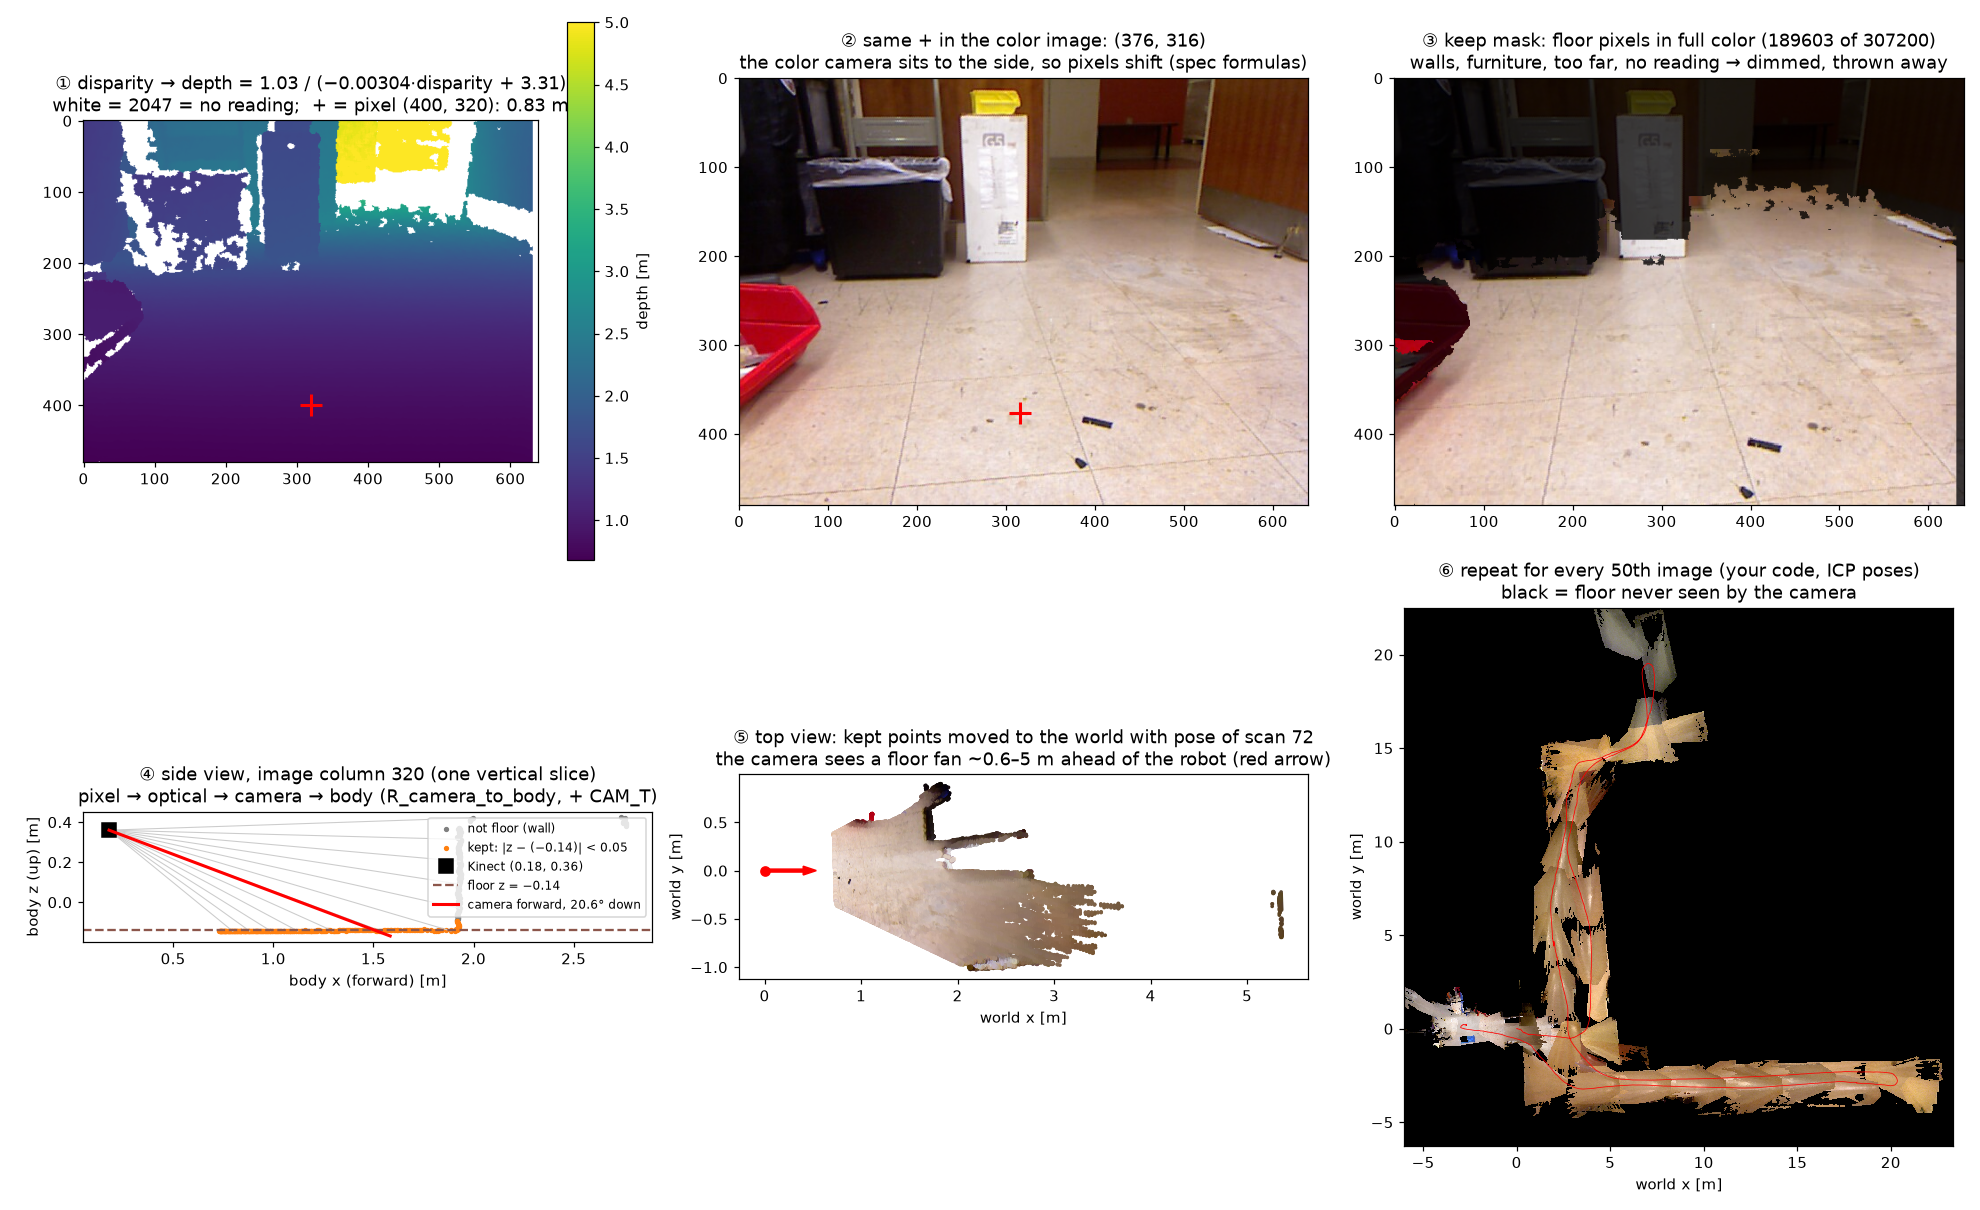
\includegraphics[width=0.9\textwidth]{figures/texture_map_explained.png}
\caption{One Kinect image through the texture pipeline (dataset 20, image 1):
(1) depth from disparity; (2) the same pixel in the color image; (3) kept
floor pixels; (4) side view of one column: rays from the tilted camera hit
the floor at $z=-0.14$\,m; (5) kept points in the world; (6) all images
painted.}
\label{fig:texture_math}
\end{figure*}

%======================================================================
\section{Results}

\begin{figure*}[t]
\centering
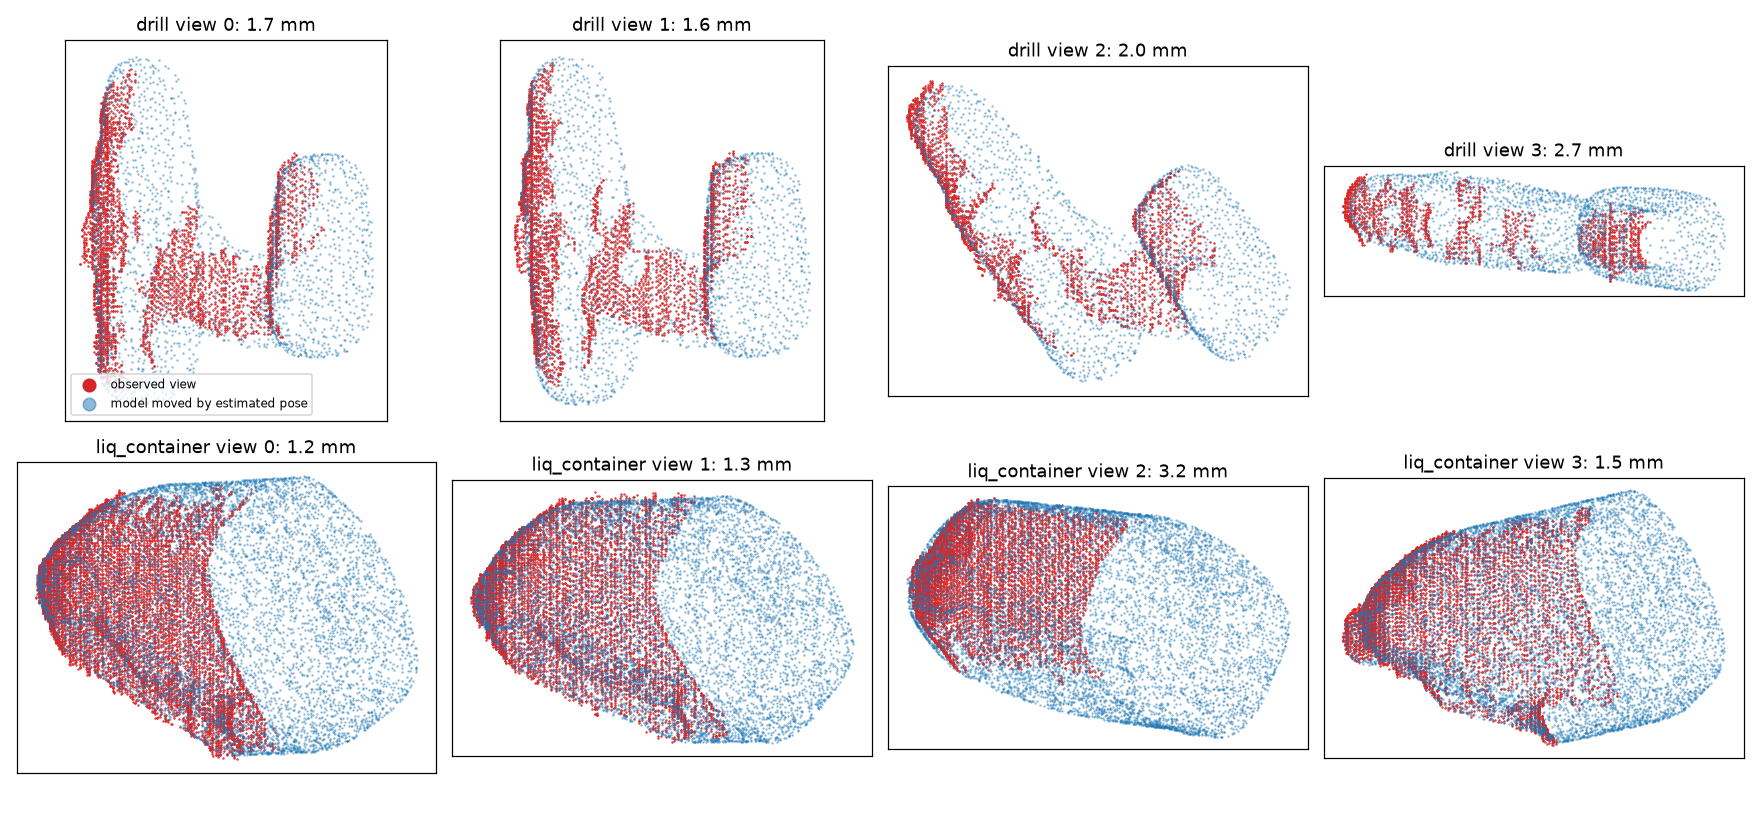
\includegraphics[width=0.85\textwidth]{figures/warmup_icp.png}
\caption{ICP warm-up, top view. Red: partial view. Blue: model moved by the
estimated pose. Title: mean point distance.}
\label{fig:warmup}
\end{figure*}

\begin{figure*}[t]
\centering
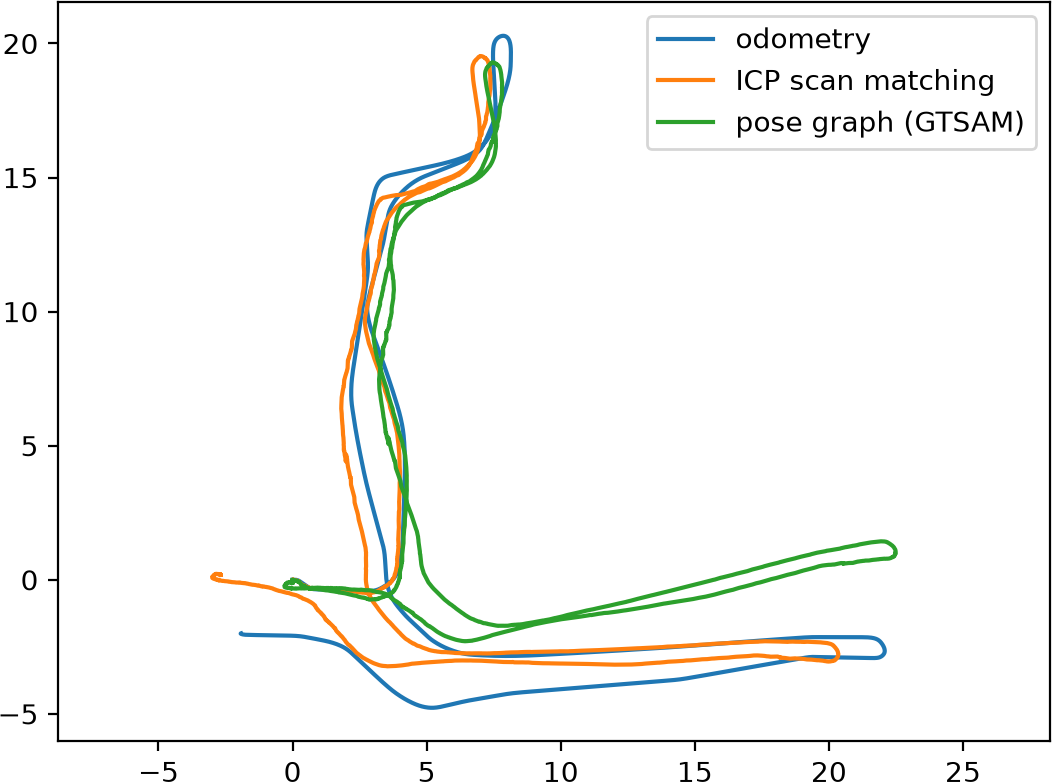
\includegraphics[width=0.48\textwidth]{figures/trajectory_20.png}\hfill
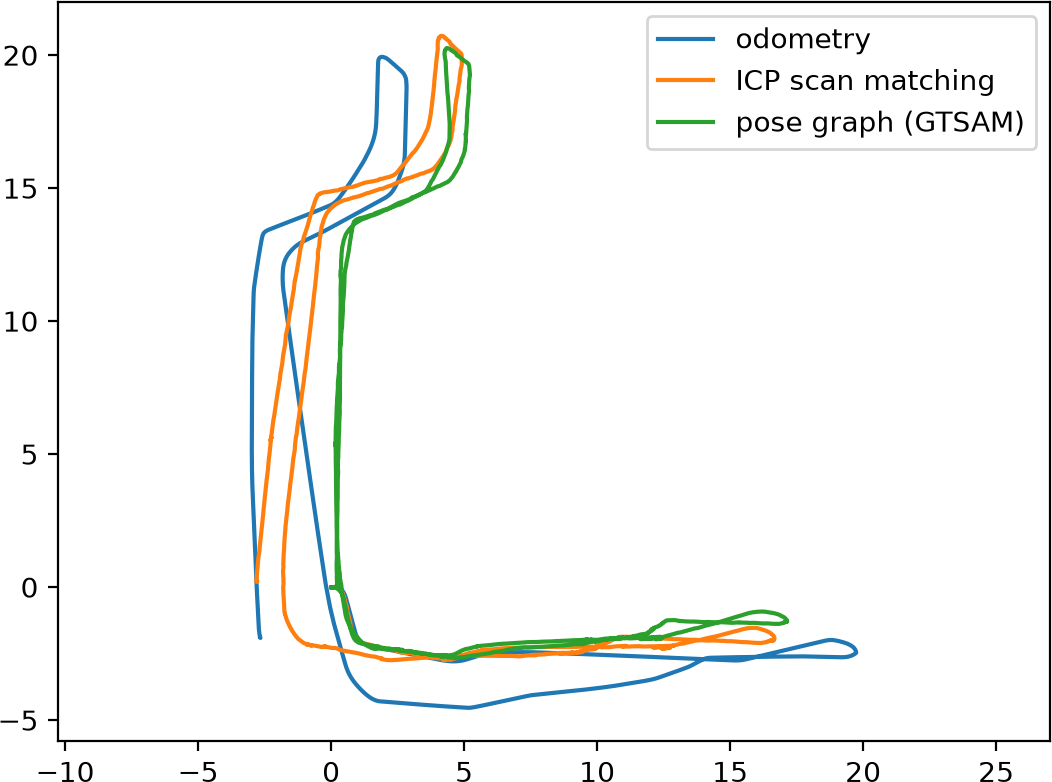
\includegraphics[width=0.48\textwidth]{figures/trajectory_21.png}
\caption{Trajectories in meters: dataset 20 (left) and 21 (right).}
\label{fig:trajectory}
\end{figure*}

\begin{figure*}[t]
\centering
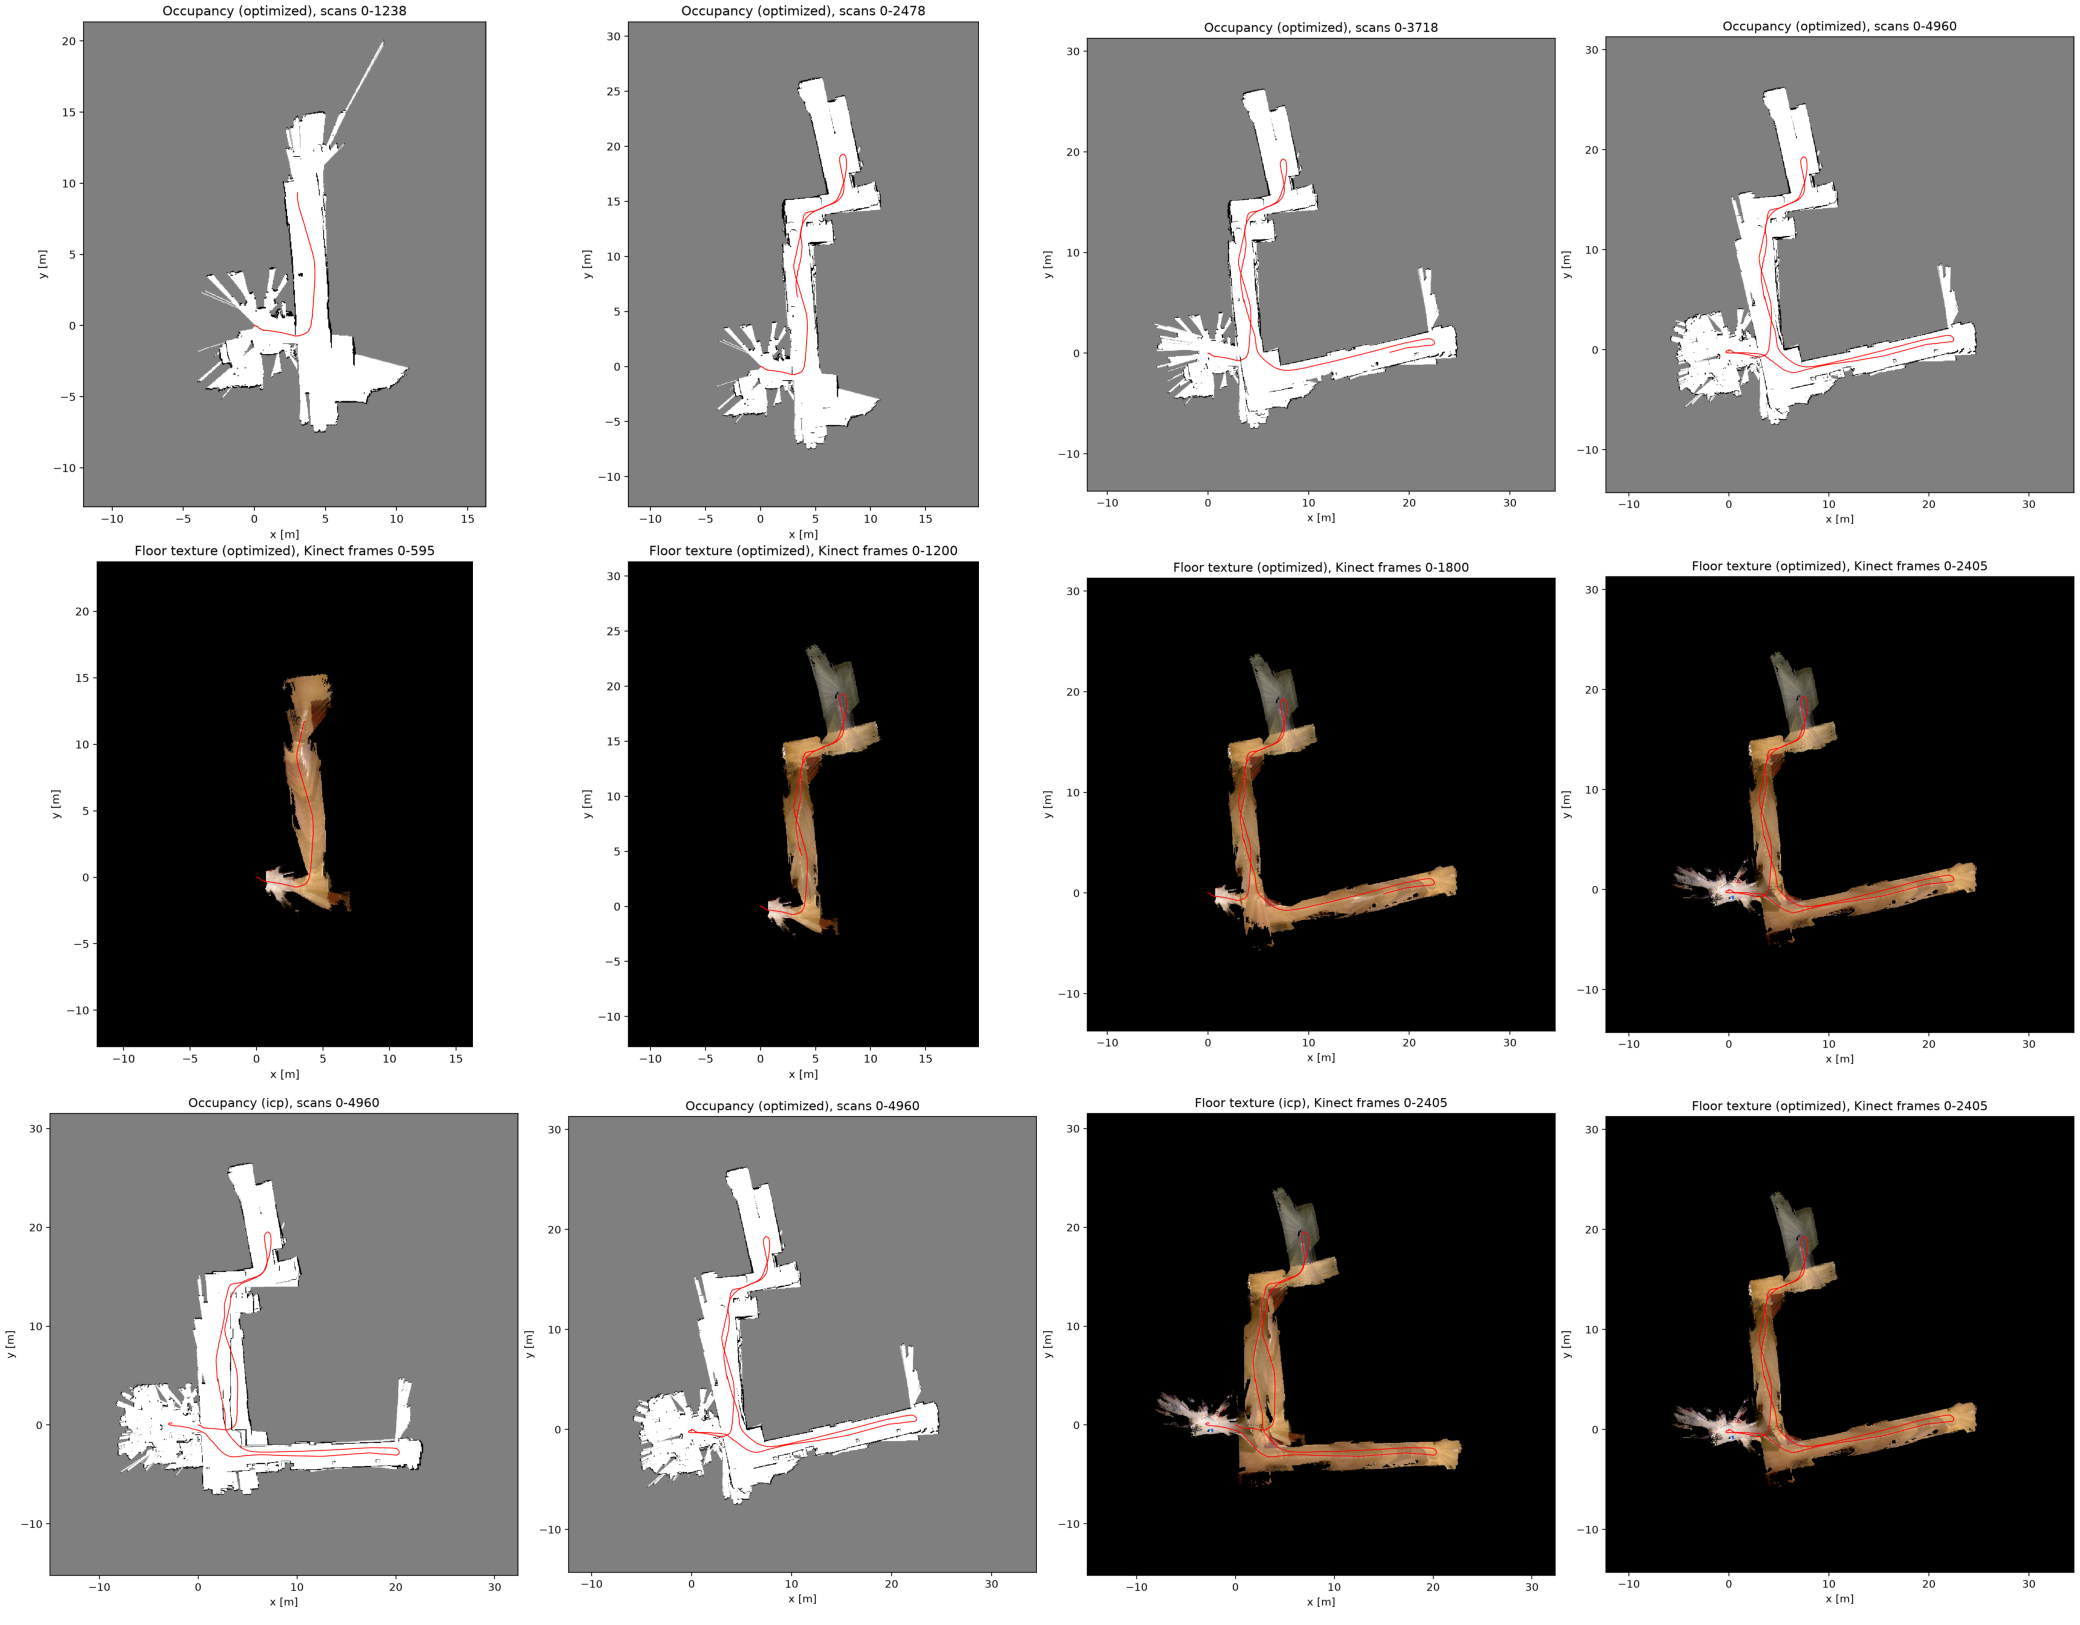
\includegraphics[width=0.95\textwidth]{figures/maps_20.png}
\caption{Dataset 20. Top: trajectory and occupancy map over time (optimized
poses; black = wall, white = free, gray = unknown, red = path so far).
Middle: floor texture over time. Bottom: final maps, ICP vs.\ optimized poses.}
\label{fig:maps20}
\end{figure*}

\begin{figure*}[t]
\centering
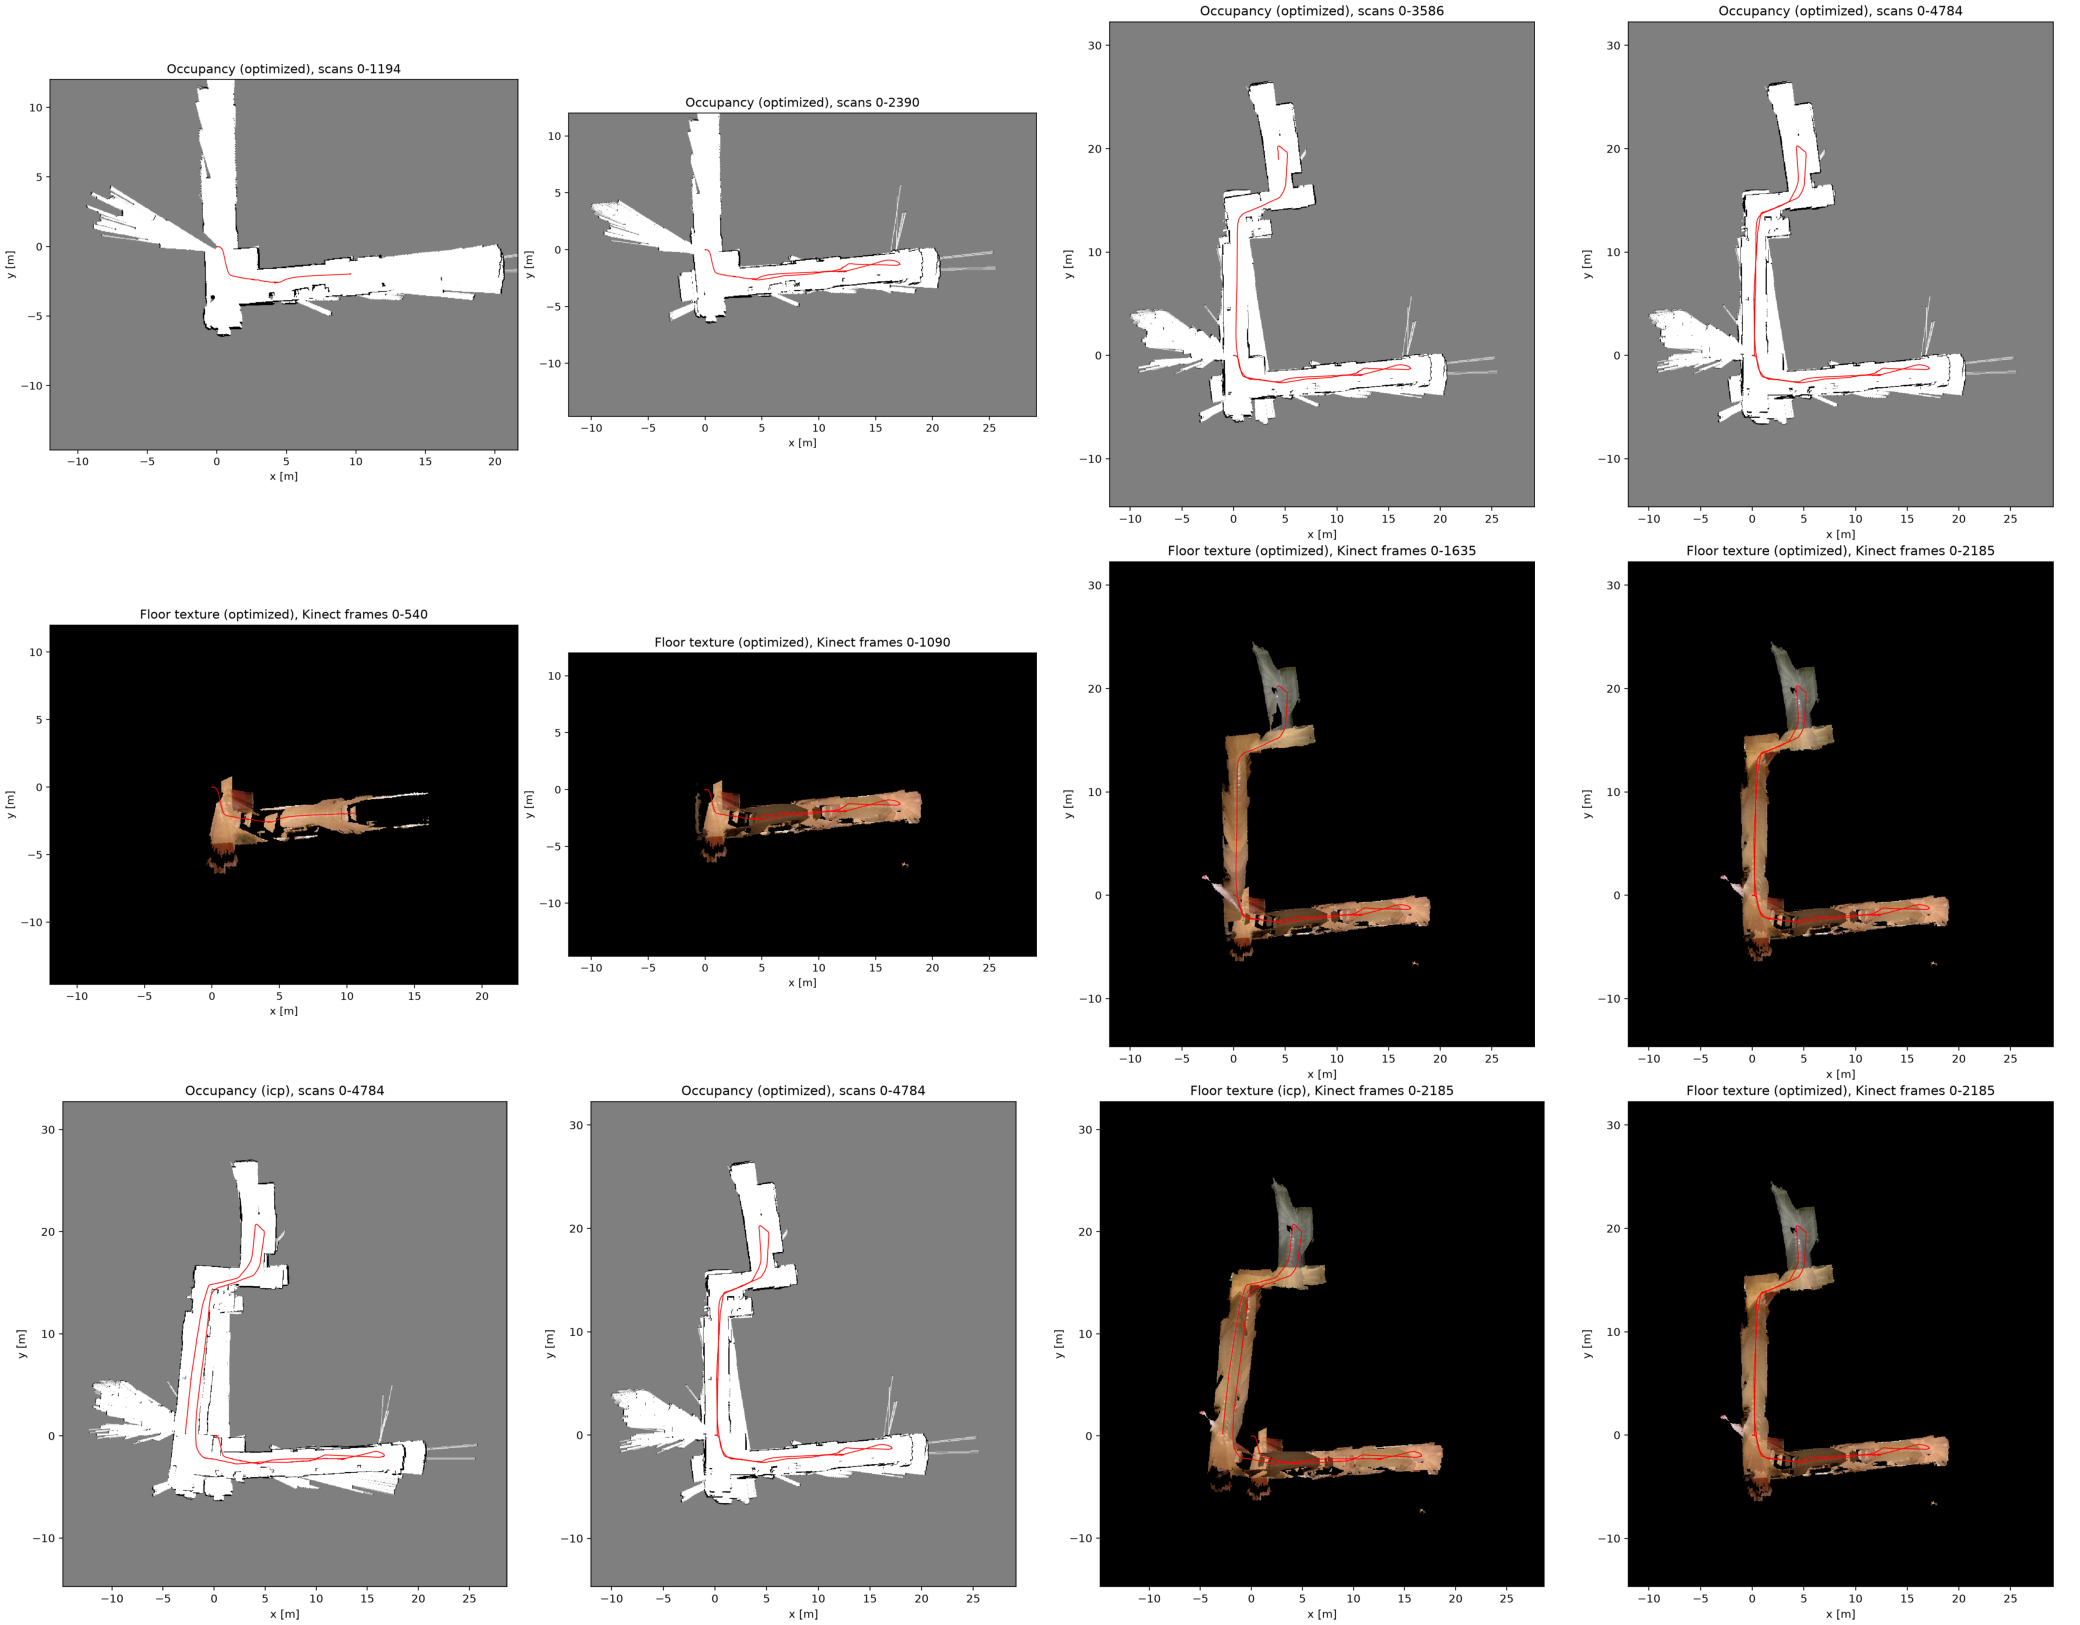
\includegraphics[width=0.95\textwidth]{figures/maps_21.png}
\caption{Dataset 21, same layout as Fig.~\ref{fig:maps20}.}
\label{fig:maps21}
\end{figure*}


\emph{ICP warm-up.} The mean distance from each view point to the model is
1.2 to 3.2\,mm for all eight views (Fig.~\ref{fig:warmup}).


\emph{Trajectories.} Without ground truth, two checks are used: the robot
returns to its start, so the gap to the start should be near 0; and
\emph{cross-pass consistency}, the median distance from a scan's points to
points seen on a different pass ($\ge500$ scans apart). A correct path makes
both passes see the same wall in the same place.

\begin{table}[t]
\caption{Trajectory quality.}
\label{tab:results}
\centering
\begin{tabular}{@{}llccc@{}}
\toprule
Data & Method & Path & Gap to start & Cross-pass \\
\midrule
20 & odometry   & 95.9\,m & 2.77\,m & 18.7\,cm \\
20 & ICP        & 95.3\,m & 2.69\,m & 10.8\,cm \\
20 & pose graph & 93.9\,m & \textbf{0.12\,m} & \textbf{2.7\,cm} \\
\midrule
21 & odometry   & 91.8\,m & 3.27\,m & 17.1\,cm \\
21 & ICP        & 96.7\,m & 2.80\,m & 11.4\,cm \\
21 & pose graph & 93.7\,m & \textbf{0.22\,m} & \textbf{1.1\,cm} \\
\bottomrule
\end{tabular}
\end{table}


ICP roughly halves the odometry error but still ends 2.7\,m from the start
(Table~\ref{tab:results}, Fig.~\ref{fig:trajectory}). The pose graph closes
the loop: 0.12 and 0.22\,m, with 2.7 and 1.1\,cm cross-pass error. It
accepted 496 fixed-interval and 121 of 875 proximity closures on dataset 20,
and 475 and 233 of 832 on dataset 21. Many proximity candidates fail because
the robot passes the same spot in the opposite direction, and a
270$^\circ$ LiDAR then sees different walls.

\begin{table}[t]
\caption{Pose graph tuning, dataset 20.}
\label{tab:tuning}
\centering
\begin{tabular}{@{}lcc@{}}
\toprule
Variant & Cross-pass & Path \\
\midrule
ICP only, no pose graph & 10.8\,cm & 95.3\,m \\
fixed-interval closures only & 11.4\,cm & 94.4\,m \\
odometry $\sigma=5$\,cm, 0.02\,rad & 1.7\,cm & \textbf{86.5\,m} \\
odometry $\sigma=1$\,cm, 0.005\,rad (used) & 2.7\,cm & 93.9\,m \\
\bottomrule
\end{tabular}
\end{table}

Fixed-interval closures alone change almost nothing, since scans 10 apart
repeat what the odometry factors already state; the proximity closures
remove the drift (Table~\ref{tab:tuning}). Loose odometry noise gives the
best cross-pass value but shortens the path by 9\,m, so path length is
checked as well.

\emph{Maps.} Figs.~\ref{fig:maps20} and~\ref{fig:maps21} show the maps over
time and ICP vs.\ optimized poses at the end. With ICP poses the return pass
is about 11\,cm off and the path end misses the start, which blurs the start
area and the walls. With optimized poses both passes overlap and the
hallways form a clean L of about 25\,m by 22\,m. Run time: scan matching
43\,s, pose graph 30\,s, occupancy map 70\,s, texture map 20\,s.



\emph{Discussion.} Odometry drifts from wheel slip and gyro bias; ICP uses
the walls but only compares nearby scans, so it still drifts; the pose
graph links scans far apart in time, which removes the drift. Three early
failures and their fixes: matching to the previous scan shrank the hallways
(keyframes), loose odometry noise bent the map (small $\sigma$), and ICP from
a bad start locked onto a wrong pose (12 initial yaws). The global rotation
of the map depends on the first hallway and cannot be checked without
ground truth.

\section*{Acknowledgment}
Claude (an AI assistant) was used as a tutor for hints and code checks
during the project, and to help draft this report from the results.

\begin{thebibliography}{3}
\bibitem{atanasov} N.~Atanasov, ``ECE 276A: Sensing \& Estimation in
Robotics,'' UC San Diego. [Online]. Available:
\url{https://natanaso.github.io/ece276a/}
\bibitem{config} ``Robot configuration,'' ECE 276A Project 2 handout
(\code{RobotConfiguration.pdf}).
\bibitem{gtsam} F.~Dellaert and GTSAM contributors, ``GTSAM.'' [Online].
Available: \url{https://github.com/borglab/gtsam}
\end{thebibliography}

\end{document}
